\subsection{Additive Manufacturing Data Types and Formats}

\begin{figure}
	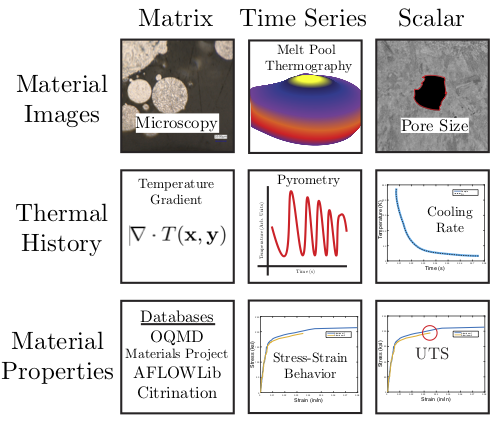
\includegraphics[width=1\linewidth]{Images/data_types.png}
	\caption{Common data types and sources in additive manufacturing research and development. This is not an exhaustive list but rather an example of how data often comes in multiple forms from multiple sources.}
	\label{datatypes}
\end{figure}

Data types and sources in additive manufacturing are as widespread as any field of engineering and science. Machine learning algorithms, however, typically operate using specific mathematical representations of data. It is important to recognize all the different sources and formats of AM data and consider how they can be coerced into use for machine learning. Examples of different AM data sources and they formats they can be collected in are shown in Figure \ref{datatypes}. Representing data in the design space properly will be a major pre-processing step for machine algorithms to be amenable to AM optimization.

Scalar data are the most commonly obtained data in materials science -- one simply needs to feel the weight of an ASME book on measured material properties to see this truth. Scalar data can include material property measurements such as strength, hardness, density and modulus. A single set of manufacturing parameters, such as heat source parameters, can also be represented as a list of scalars. Desired models in AM research include models of the relationships between material properties and manufacturing parameters. In these cases, the machine inputs will most often be represented as a vector, such as
\begin{equation}
\begin{split}
	\mathbf{x} & = \text{[} \text{Machine Input 1, Machine Input 2,} \hdots  \\
		& \hdots \text{, Machine Input } n \text{]} \\
	\label{vector}
\end{split}
\end{equation}
out of $n$ many scalar machine inputs. Vector representations of the design space are useful in determining manufacturing conditions which will result in similar results, as well as in building regression models of the AM process.


Another common data type often represented by vectors is \textit{time series} data. Time series data are usually measured during the manufacturing process. Highly desired time series data collected during AM are temperature histories; others include videos, spectroscopy, and part deformation and strain. These data can sometimes be used as-is, or operations can be performed to extract scalar data values from the time series. Scalar statistical values such as the maximum, minimum, mean, and standard deviation of a time series signal can be equally useful in machine learning applications. Signal processing of time series data is also an active area of machine learning research which seeks to extract the most useful information from a time series. Pre-processing time series data can result in useful machine learning inputs; separately, signal processing algorithms have been used to reduce the amount of data required for machine learning to be successful \cite{Candes2008}.

Matrices are perhaps the most diverse type of data used in terms of the range of materials science information that they can convey. Large datasets of scalar values measured multiple times will often be represented by a matrix where the columns represent each individual measurement type and the rows are repeated measurements of that value, usually for different samples. Representing this collection of scalar measurements as as a matrix can be useful; one example would be
\begin{equation}
	\mathbf{X} = \begin{bmatrix} x_{1,1} & x_{1,2} & \hdots & x_{1,m} \\
						x_{2,1} & x_{2,2} & \hdots & x_{2,m} \\
						\vdots & \vdots & \vdots & \vdots \\
						x_{n,1} & x_{n,2} & \hdots & x_{n,m} \\
				\end{bmatrix}
	\label{matrix}
\end{equation}
where the columns of $\mathbf{X}$ represent the different design space considerations being made, out of $m$, and there have been $n$ repeated measurements of each. Time series data can be represented in a similar way, with each column being a point in time and each row being a different measurement of the time series data. \footnote{It is important to note that the row and column definitions given here are not concrete; indeed, the columns could be repeated measurements and the rows could represent different measurement types. If a machine learning algorithm is sensitive to the row-column definitions, the solution is as easy as taking a transpose.}

Images are also most often represented as matrices. Each entry in the matrix represents something about a corresponding pixel in the image: it could be a grayscale intensity, it could be one of the three RGB channel values, it could be a binary value, etc. Almost all image processing algorithms discussed in this review rely on a matrix representation of images. There are many toolboxes available, both free and commercial, which can pre-process images into the correct form for machine learning algorithms. Examples include the MATLAB Computer Vision Toolbox and the C++/Python OpenCV libraries.

Thus far, various manners of formatting data for machine learning has been discussed. The examples given have been formats for data measured directly from an experiment. While many machine learning algorithms can operate directly on machine inputs and processing outputs, it can be equally useful to measure the relationship between data points, instead of focusing on the data points themselves. \textit{Covariance} is measured between two data points $\kappa (\mathbf{x},\mathbf{x}')$, instead of being a property of a single data point. The function $\kappa(\cdot,\cdot)$ is often referred to as a kernel function. The covariance between data points encodes cross-correlated information within the design space. In most cases, kernel functions assess the similarity of design space coordinates. Ways of calculating covariance are many and varied and will be explicitly defined where they are used. The nature of \textit{why} covariance is a useful tool for machine learning algorithms is slightly more complex than this review article allows; however, some of the most powerful and useful machine learning applications in materials science have relied on the calculation of covariance between design space coordinates. Readers who are seeking more information on the use of covariance in machine learning are directed to \cite{KernelMethod}.